\documentclass[aspectratio=169, 11pt]{beamer}

\usetheme{Madrid}
\usecolortheme{default}
\useinnertheme{rectangles}
\setbeamertemplate{navigation symbols}{}
\setbeamertemplate{footline}[frame number]

\usepackage{amsmath,amssymb,bm}
\usepackage{graphicx}
\usepackage{booktabs}
\usepackage{hyperref}
\usepackage{tikz}
\usepackage{xcolor}

\graphicspath{{../figures/}{../results/}}

% Custom colors
\definecolor{safegreen}{RGB}{50,190,50}
\definecolor{stochblue}{RGB}{77,128,218}
\definecolor{robpurple}{RGB}{153,51,153}
\definecolor{dangerred}{RGB}{230,64,64}

\title[RVD Tumbling Target]{Reachability-Aware Guidance for Approach\\to a Tumbling Uncooperative Target\\with Time-Varying LOS Constraints}
\author{Author~1 \and Author~2}
\institute{Affiliation}
\date{IAC 2026 -- Antalya, T\"urkiye\\5--9 October 2026}

\begin{document}

% ============================================================
% MAIN SLIDES (15)
% ============================================================

% --- Slide 1: Title ---
\begin{frame}
\titlepage
\end{frame}

% --- Slide 2: Motivation & Problem ---
\begin{frame}{Motivation \& Problem Statement}
\begin{columns}[T]
\column{0.55\textwidth}
\textbf{Challenge:}
\begin{itemize}
    \item Autonomous rendezvous with a \textbf{tumbling}, uncooperative target
    \item Docking corridor (LOS cone) \textbf{rotates with target body}
    \item Chaser must maintain LOS feasibility \textbf{at all times}
\end{itemize}
\vspace{0.3cm}
\textbf{Key question:}\\
\emph{From which initial states can the chaser safely approach?}

\column{0.42\textwidth}
\centering
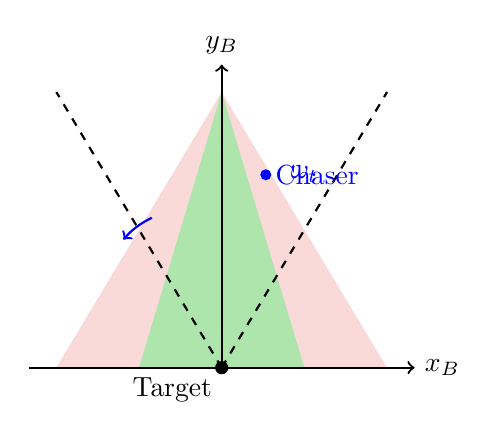
\begin{tikzpicture}[scale=0.7]
    \fill[dangerred!20] (-3,0) -- (0,5) -- (3,0) -- cycle;
    \fill[safegreen!40] (-1.5,0) -- (0,5) -- (1.5,0) -- cycle;
    \draw[->, thick] (0,0) -- (0,5.5) node[above] {$y_B$};
    \draw[->, thick] (-3.5,0) -- (3.5,0) node[right] {$x_B$};
    \draw[thick, dashed] (0,0) -- (3,5);
    \draw[thick, dashed] (0,0) -- (-3,5);
    \draw[->, blue, thick, rotate=25] (0,3) arc (90:115:1.5);
    \node[blue] at (1.5,3.5) {$\omega_t$};
    \fill[black] (0,0) circle (0.12) node[below left] {Target};
    \fill[blue] (0.8,3.5) circle (0.1) node[right] {Chaser};
\end{tikzpicture}
\end{columns}
\end{frame}

% --- Slide 3: Contributions ---
\begin{frame}{Paper Contributions}
\begin{enumerate}
    \item \textbf{Analytical reachability hierarchy}\\
    Four nested certified feasibility regions:\\
    $\mathcal{X}_{\text{rob}} \subseteq \mathcal{X}_{\text{stoch}} \subseteq \mathcal{X}_{\text{nom}} \subseteq \mathcal{X}_{\text{MC}}$

    \vspace{0.3cm}
    \item \textbf{Physically honest CWH propagation}\\
    No reference blending or state projection\\
    Exact discrete state-transition matrix $\Phi(\tau)$

    \vspace{0.3cm}
    \item \textbf{Parametric feasibility maps}\\
    20 sweep cases: $\omega_t \in \{1,...,5\}$ deg/s $\times$ $a_{\max} \in \{0.2,...,0.02\}$ m/s$^2$

    \vspace{0.3cm}
    \item \textbf{MC validation}\\
    195+ closed-loop simulations per parameter combination
\end{enumerate}
\end{frame}

% --- Slide 4: CWH Dynamics ---
\begin{frame}{Dynamics: CWH Relative Motion}
\textbf{State:} $\mathbf{x} = [x, y, z, \dot{x}, \dot{y}, \dot{z}]^\top$ in LVLH

\vspace{0.2cm}
\textbf{Continuous CWH:}
\begin{align*}
\ddot{x} &= 3n^2 x + 2n\dot{y} + a_x \\
\ddot{y} &= -2n\dot{x} + a_y \\
\ddot{z} &= -n^2 z + a_z
\end{align*}

\textbf{Discrete (exact matrix exponential):}
$$\mathbf{x}_{k+1} = \Phi(\Delta t)\,\mathbf{x}_k + B_d(\Delta t)\,\mathbf{u}_k$$

\vspace{0.2cm}
\begin{block}{Key principle}
Truth propagation uses \textbf{only} CWH + commanded acceleration.\\
No reference blending, no state projection $\Rightarrow$ physically honest feasibility claims.
\end{block}
\end{frame}

% --- Slide 5: LOS Corridor ---
\begin{frame}{Time-Varying LOS Corridor}
\begin{columns}[T]
\column{0.50\textwidth}
\textbf{Body-frame constraints:}
$$A_c\, \mathbf{p}_B \leq b_c$$

\vspace{0.1cm}
5 half-space inequalities:
\begin{itemize}
    \item $y_B \geq r_h$ (hold distance)
    \item $|x_B| \leq x_0 + c_x(y_B - r_h)$ (lateral cone)
    \item $|z_B| \leq z_0 + c_z(y_B - r_h)$ (out-of-plane)
\end{itemize}

\vspace{0.3cm}
\textbf{Body $\leftrightarrow$ LVLH:}
$$\mathbf{p}_B = R_z(-\omega_t t)\,\mathbf{p}_L$$

Constraints \textbf{rotate} in LVLH frame!

\column{0.47\textwidth}
\centering
% Placeholder for LOS figure
\fbox{\parbox{0.9\textwidth}{\centering\vspace{2cm}
\textit{LOS cone schematic}\\
\textit{(rotating in LVLH)}
\vspace{2cm}}}
\end{columns}
\end{frame}

% --- Slide 6: Safe-Start Analysis ---
\begin{frame}{Safe-Start Region: Erosion Model}
\begin{columns}[T]
\column{0.50\textwidth}
\textbf{Directional per-constraint erosion:}
$$\delta_i = \frac{(\dot{s}_i^-)^2}{2\,a_{\max}}$$

\begin{itemize}
    \item $\dot{s}_i$: constraint slack rate from rotation
    \item Only negative rates cause erosion
    \item Creates \textbf{asymmetric} safe region
\end{itemize}

\vspace{0.3cm}
\textbf{Synchronization range bound:}
$$r < r_{\text{sync}} = \frac{2\,a_{\max}}{\omega_t^2}$$

\column{0.47\textwidth}
\textbf{Physical interpretation:}\\[0.2cm]
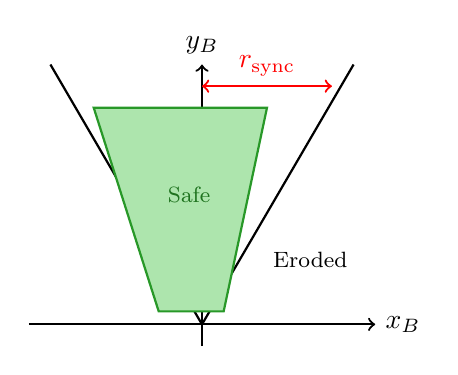
\begin{tikzpicture}[scale=0.55]
    \draw[->, thick] (-4,0) -- (4,0) node[right] {$x_B$};
    \draw[->, thick] (0,-0.5) -- (0,6) node[above] {$y_B$};
    \draw[thick] (0,0) -- (3.5,6);
    \draw[thick] (0,0) -- (-3.5,6);
    \fill[safegreen!40] (-1,0.3) -- (-2.5,5) -- (1.5,5) -- (0.5,0.3) -- cycle;
    \draw[safegreen!80!black, thick] (-1,0.3) -- (-2.5,5) -- (1.5,5) -- (0.5,0.3) -- cycle;
    \draw[<->, red, thick] (0,5.5) -- node[above] {$r_{\text{sync}}$} (3,5.5);
    \node[safegreen!60!black] at (-0.3,3) {\footnotesize Safe};
    \node at (2.5,1.5) {\footnotesize Eroded};
\end{tikzpicture}

The safe region \textbf{tilts} toward the downstream side of rotation.
\end{columns}
\end{frame}

% --- Slide 7: Feasibility Hierarchy ---
\begin{frame}{Hierarchy of Certified Feasibility Sets}
\begin{center}
\large
$\mathcal{X}_{\text{rob}} \;\subseteq\; \mathcal{X}_{\text{stoch}} \;\subseteq\; \mathcal{X}_{\text{nom}} \;\subseteq\; \mathcal{X}_{\text{MC}}$
\end{center}

\vspace{0.2cm}
\begin{columns}[T]
\column{0.48\textwidth}
\begin{block}{\textcolor{safegreen}{Nominal} $\mathcal{X}_{\text{nom}}$}
Perfect model, zero disturbance.\\
Erosion $\delta_i$ + sync bound $r_{\text{sync}}$.
\end{block}

\begin{block}{\textcolor{stochblue}{Stochastic} $\mathcal{X}_{\text{stoch}}$ (95\%)}
Gaussian noise $\mathbf{w}_k \sim \mathcal{N}(0, W)$.\\
Tighten by $z_{1-\alpha/n_c} \cdot \sigma_i$.
\end{block}

\column{0.48\textwidth}
\begin{block}{\textcolor{robpurple}{Robust} $\mathcal{X}_{\text{rob}}$}
Bounded $\|\mathbf{w}_k\|_\infty \leq w_{\max}$.\\
Tighten by $\sum_j h_{\mathcal{W}}(\mathbf{a}_i^\top A^j)$.
\end{block}

\begin{block}{\textcolor{safegreen!50}{MC} $\mathcal{X}_{\text{MC}}$}
Empirical: 195+ closed-loop simulations.\\
No formal guarantees.
\end{block}
\end{columns}

\vspace{0.3cm}
\centering
\textbf{``Price of certification''}: region shrinks as guarantees strengthen.
\end{frame}

% --- Slide 8: Nominal Results ---
\begin{frame}{Nominal Reachability Results}
\begin{center}
\includegraphics[width=0.88\textwidth]{nominal_forward_grid.png}
\end{center}
\vspace{-0.3cm}
\small Green = certified safe, Blue = inside cone (unsafe), Red = outside cone
\end{frame}

% --- Slide 9: Stochastic Results ---
\begin{frame}{Stochastic Reachability (95\% Confidence)}
\begin{center}
\includegraphics[width=0.88\textwidth]{stochastic_grid.png}
\end{center}
\vspace{-0.3cm}
\small $\alpha = 0.05$, Bonferroni-corrected. Regions shrink vs.\ nominal due to noise tightening.
\end{frame}

% --- Slide 10: Robust Results ---
\begin{frame}{Robust Reachability (Worst-Case)}
\begin{center}
\includegraphics[width=0.88\textwidth]{robust_grid.png}
\end{center}
\vspace{-0.3cm}
\small Most conservative: guarantees feasibility for ALL disturbances in $\mathcal{W}$.
\end{frame}

% --- Slide 11: Nested Comparison ---
\begin{frame}{Nested Comparison: All Three Methods}
\begin{center}
\includegraphics[width=0.88\textwidth]{comparison_grid.png}
\end{center}
\vspace{-0.3cm}
\small \textcolor{safegreen}{Nominal} $\supset$ \textcolor{stochblue}{Stochastic} $\supset$ \textcolor{robpurple}{Robust}: hierarchy verified for all 20 combinations.
\end{frame}

% --- Slide 12: MC Validation ---
\begin{frame}{Monte Carlo Validation}
\begin{columns}[T]
\column{0.55\textwidth}
\begin{itemize}
    \item 195 initial conditions per combo
    \item Full MPC closed-loop simulation
    \item Nonlinear ECI truth dynamics (2-body + J2)
    \item 20 parameter combinations = 3,900 runs
\end{itemize}

\vspace{0.3cm}
\textbf{Validation:}
$$\mathcal{X}_{\text{nom}} \subseteq \mathcal{X}_{\text{MC}}$$
No analytically certified point lies outside the MC-safe region.

\column{0.42\textwidth}
\fbox{\parbox{0.9\textwidth}{\centering\vspace{2.5cm}
\textit{MC heatmap}\\
\textit{(from fig\_mc\_sweep\_grid.png)}
\vspace{2.5cm}}}
\end{columns}
\end{frame}

% --- Slide 13: Area Ratios ---
\begin{frame}{Area Ratio Summary}
\begin{center}
\begin{tabular}{l c c c c}
\toprule
& \multicolumn{4}{c}{Fraction of LOS cone area} \\
\cmidrule(lr){2-5}
Combination & Nominal & Stochastic & Robust & MC \\
\midrule
$\omega$=1, $a$=0.20 & high & $<$ nom & $<$ stoch & $>$ nom \\
$\omega$=3, $a$=0.10 & medium & medium & small & $>$ nom \\
$\omega$=5, $a$=0.02 & $\approx$0 & 0 & 0 & $\approx$0 \\
\bottomrule
\end{tabular}
\end{center}

\vspace{0.5cm}
\begin{block}{Key insight}
\textbf{Feasibility governed by} $a_{\max}/\omega_t^2$. When $r_{\text{sync}} < y_{\min}$, no initial condition is feasible regardless of method.
\end{block}
\end{frame}

% --- Slide 14: Key Findings ---
\begin{frame}{Key Findings}
\begin{enumerate}
    \item \textbf{Inclusion hierarchy verified:}\\
    $\mathcal{X}_{\text{rob}} \subseteq \mathcal{X}_{\text{stoch}} \subseteq \mathcal{X}_{\text{nom}} \subseteq \mathcal{X}_{\text{MC}}$ holds for all 20 cases.

    \vspace{0.3cm}
    \item \textbf{Synchronization radius is the key parameter:}\\
    $r_{\text{sync}} = 2a_{\max}/\omega_t^2$ bounds the feasible approach region.

    \vspace{0.3cm}
    \item \textbf{Physical honesty matters:}\\
    Double-integrator models give artificially optimistic results.\\
    CWH along-track coupling is the dominant real-world challenge.

    \vspace{0.3cm}
    \item \textbf{Analytical methods are $>$100$\times$ faster than MC}\\
    while providing formal safety certificates.
\end{enumerate}
\end{frame}

% --- Slide 15: Conclusions & Future Work ---
\begin{frame}{Conclusions \& Future Work}
\textbf{Conclusions:}
\begin{itemize}
    \item Reachability-aware guidance with \textbf{four-level certification hierarchy}
    \item Directional erosion + sync bound = conservative but physically meaningful
    \item All results reproducible from a single MATLAB command
\end{itemize}

\vspace{0.3cm}
\textbf{Future work:}
\begin{itemize}
    \item Formal viability-kernel computation (exact polytope propagation)
    \item Multi-phase approach: LVLH $\to$ body-frame transition at $r_{\text{sync}}$
    \item Extension to 3D tumble (general attitude kinematics)
    \item Real-time onboard reachability assessment
\end{itemize}

\vspace{0.3cm}
\centering
\textbf{Thank you!} \quad Questions?
\end{frame}


% ============================================================
% BACKUP SLIDES (20)
% ============================================================
\appendix

\begin{frame}
\centering
\vspace{2cm}
{\Huge \textbf{Backup Slides}}
\vspace{1cm}
\end{frame}

% --- B1: CWH STM Details ---
\begin{frame}{Backup: CWH State-Transition Matrix}
\small
$$\Phi(\tau) = \begin{bmatrix}
4 - 3c & 0 & 0 & s/n & 2(1-c)/n & 0 \\
6(s - n\tau) & 1 & 0 & -2(1-c)/n & (4s - 3n\tau)/n & 0 \\
0 & 0 & c & 0 & 0 & s/n \\
3ns & 0 & 0 & c & 2s & 0 \\
-6n(1-c) & 0 & 0 & -2s & 4c-3 & 0 \\
0 & 0 & -ns & 0 & 0 & c
\end{bmatrix}$$

$$B_d(\tau) = \begin{bmatrix}
(1-c)/n^2 & 2(n\tau-s)/n^2 & 0 \\
-2(n\tau-s)/n^2 & (4(1-c)-1.5n^2\tau^2)/n^2 & 0 \\
0 & 0 & (1-c)/n^2 \\
s/n & 2(1-c)/n & 0 \\
-2(1-c)/n & (4s-3n\tau)/n & 0 \\
0 & 0 & s/n
\end{bmatrix}$$

where $c = \cos(n\tau)$, $s = \sin(n\tau)$.
\end{frame}

% --- B2: LOS Constraint Matrix ---
\begin{frame}{Backup: LOS Constraint Formulation}
\textbf{Five half-space constraints in body frame:}
$$A_c = \begin{bmatrix}
0 & -1 & 0 \\ 1 & -c_x & 0 \\ -1 & -c_x & 0 \\ 0 & -c_z & 1 \\ 0 & -c_z & -1
\end{bmatrix}, \quad
b_c = \begin{bmatrix}
-r_h \\ x_0 - c_x r_h \\ x_0 - c_x r_h \\ z_0 - c_z r_h \\ z_0 - c_z r_h
\end{bmatrix}$$

\textbf{Parameters:} $c_x = c_z = 1.5$, $x_0 = z_0 = 2.5$ m, $r_h = 0.5$ m

\vspace{0.3cm}
\textbf{In LVLH at time $t$:}
$$A_c\, R_z(-\omega_t t)\, \mathbf{p}_L \leq b_c$$
\end{frame}

% --- B3: Body-LVLH Transform ---
\begin{frame}{Backup: Body--LVLH Transform}
\textbf{Position:}
$$\mathbf{r}_B = R_z(-\theta)\,\mathbf{r}_L, \quad \theta = \omega_t t$$

\textbf{Velocity (transport theorem):}
\begin{align*}
\mathbf{v}_B &= R_z(-\theta)\,\mathbf{v}_L - \boldsymbol{\omega} \times \mathbf{r}_B \\
\mathbf{v}_L &= R_z(\theta)\left(\mathbf{v}_B + \boldsymbol{\omega} \times \mathbf{r}_B\right)
\end{align*}

\textbf{Implication:} At range $r$, body-stationary requires LVLH co-rotation velocity $v_{\text{corot}} = \omega_t r$.
\end{frame}

% --- B4: Erosion Derivation ---
\begin{frame}{Backup: Erosion Derivation}
\textbf{Rotation-induced apparent velocity:}
$$\mathbf{v}_{\text{rot}} = [\omega_t y_B,\; -\omega_t x_B,\; 0]^\top$$

\textbf{Constraint slack rate:}
$$\dot{s}_i = -\mathbf{a}_i^\top \mathbf{v}_{\text{rot}}$$

\textbf{If $\dot{s}_i < 0$ (margin shrinking):}
\begin{itemize}
    \item Settling time: $t_s = |\dot{s}_i| / a_{\max}$
    \item Margin consumed: $\delta_i = \frac{1}{2}\dot{s}_i^2 / a_{\max}$
\end{itemize}

\textbf{Safe if:} $s_i - \delta_i > 0$ for all constraints $i$.

\vspace{0.3cm}
This creates asymmetric safe regions: for $\omega_t > 0$ (CCW), the right-hand cone boundary erodes faster.
\end{frame}

% --- B5: Sync Range Derivation ---
\begin{frame}{Backup: Synchronization Range Derivation}
\textbf{At range $r$:}
\begin{itemize}
    \item Apparent rotational speed: $v_{\text{rot}} = \omega_t r$
    \item Braking distance: $d_{\text{brake}} = \frac{v_{\text{rot}}^2}{2\,a_{\max}} = \frac{\omega_t^2 r^2}{2\,a_{\max}}$
\end{itemize}

\textbf{Require} $d_{\text{brake}} < r$:
$$\frac{\omega_t^2 r^2}{2\,a_{\max}} < r \quad\Rightarrow\quad r < \frac{2\,a_{\max}}{\omega_t^2} = r_{\text{sync}}$$

\vspace{0.3cm}
\begin{center}
\begin{tabular}{ccc}
\toprule
$\omega_t$ (deg/s) & $a_{\max}$ (m/s$^2$) & $r_{\text{sync}}$ (m) \\
\midrule
1 & 0.10 & 656.6 \\
3 & 0.10 & 72.9 \\
5 & 0.10 & 26.3 \\
1 & 0.02 & 131.3 \\
\bottomrule
\end{tabular}
\end{center}
\end{frame}

% --- B6: Stochastic Tightening ---
\begin{frame}{Backup: Stochastic Constraint Tightening}
\textbf{Process noise model:}
$$\mathbf{x}_{k+1} = \Phi\,\mathbf{x}_k + B_d\,\mathbf{u}_k + \mathbf{w}_k, \quad \mathbf{w}_k \sim \mathcal{N}(0, W)$$

\textbf{Accumulated covariance:}
$$\Sigma_N = \sum_{j=0}^{N-1} \Phi^j W (\Phi^j)^\top$$

\textbf{Chance constraint:} $\Pr(A_c\,\mathbf{x}_k \leq b_c) \geq 1 - \alpha$

\textbf{Tightening (Bonferroni):}
$$b_i^{\text{tight}} = b_i - \Phi^{-1}\!\left(1 - \tfrac{\alpha}{n_c}\right) \cdot \sqrt{\mathbf{a}_i^\top \Sigma_N \mathbf{a}_i}$$

With $\alpha = 0.05$, $n_c = 9$: $z_{0.9944} \approx 2.54$.
\end{frame}

% --- B7: Robust Tightening ---
\begin{frame}{Backup: Robust Constraint Tightening}
\textbf{Bounded disturbance:}
$$\mathbf{w}_k \in \mathcal{W} = \{\mathbf{w} : \|\mathbf{w}\|_\infty \leq w_{\max}\}$$

\textbf{Worst-case accumulated tightening:}
$$\Delta_i^{\text{rob}} = \sum_{j=0}^{N-1} \max_{\mathbf{w} \in \mathcal{W}} \mathbf{a}_i^\top \Phi^j \mathbf{w} = \sum_{j=0}^{N-1} \|\mathbf{a}_i^\top \Phi^j\|_1 \cdot w_{\max}$$

\textbf{Tightened constraint:}
$$s_i(\mathbf{x}) > \delta_i^{\text{nom}} + \Delta_i^{\text{rob}}$$

This is the most conservative: guarantees for \emph{all} disturbance sequences.
\end{frame}

% --- B8: MPC QP Formulation ---
\begin{frame}{Backup: MPC Quadratic Program}
\textbf{Decision variables:} $\mathbf{z} = [\mathbf{x}_0;\,...\,;\mathbf{x}_N;\,\mathbf{u}_0;\,...\,;\mathbf{u}_{N-1}]$

\textbf{Cost:}
$$\min_{\mathbf{z}} \sum_{k=0}^{N-1} \left(\|\mathbf{x}_k - \mathbf{x}^{\text{ref}}\|_Q^2 + \|\mathbf{u}_k\|_R^2 + \|\Delta\mathbf{u}_k\|_{R_{\Delta}}^2\right) + \|\mathbf{x}_N - \mathbf{x}^{\text{ref}}\|_{Q_N}^2$$

\textbf{Subject to:}
\begin{itemize}
    \item Dynamics: $\mathbf{x}_{k+1} = \Phi\,\mathbf{x}_k + B_d\,\mathbf{u}_k$
    \item Input bounds: $\|\mathbf{u}_k\|_\infty \leq a_{\max}$
    \item LOS cone: $A_c\,R_z(-\theta_k)\,\mathbf{x}_k^{[1:3]} \leq b_c$
\end{itemize}

\textbf{Solver:} OSQP (warm-started, polished).\\
\textbf{Size:} 366 variables, 735 constraints per step.
\end{frame}

% --- B9: Three-Regime Controller ---
\begin{frame}{Backup: Three-Regime Controller}
\begin{enumerate}
    \item \textbf{Far approach} ($r > r_{\text{sync}}$):\\
    LVLH-frame PD tracking, velocity limited by $v_{\text{achv}} = \min(a_{\max}t/2, v_{\max})$

    \vspace{0.3cm}
    \item \textbf{Close approach} ($r \leq r_{\text{sync}}$):\\
    Body-frame PD tracking with CWH feedforward

    \vspace{0.3cm}
    \item \textbf{Hold} ($|r - r_h| < \epsilon$, $v < v_{\text{switch}}$):\\
    Synchronized station-keeping with stiff PD + CWH gravity-gradient compensation:
    $$\mathbf{a}_{\text{ff}} = -\begin{bmatrix} 3n^2 x + 2n\dot{y} \\ -2n\dot{x} \\ -n^2 z \end{bmatrix}$$
\end{enumerate}
\end{frame}

% --- B10: Along-Track Coupling ---
\begin{frame}{Backup: CWH Along-Track Coupling}
The $(2,1)$ element of $\Phi(\tau)$ contains the \textbf{secular term}:
$$\Phi_{21} = 6(s - n\tau)$$

This means any radial offset $x$ produces unbounded along-track drift:
$$\Delta y \approx 6n(s - n\tau)\,x$$

\textbf{Impact:}
\begin{itemize}
    \item At 195 m range, even small radial offsets cause large along-track acceleration
    \item Double-integrator models miss this entirely $\Rightarrow$ artificially optimistic
    \item Controller must actively compensate CWH coupling
\end{itemize}

This is why the synchronization radius alone is not sufficient --- the controller must also manage orbital dynamics coupling.
\end{frame}

% --- B11: Physical Honesty ---
\begin{frame}{Backup: Why Physical Honesty Matters}
\textbf{Earlier implementations used:}
\begin{itemize}
    \item Double-integrator truth dynamics
    \item Reference blending / state projection
    \item ``Phantom'' $\Delta v$ from state teleportation
\end{itemize}

\textbf{Result:} Up to 80\% of fuel expenditure was unphysical!

\vspace{0.3cm}
\textbf{Example:} $\omega_t = 10$ deg/s, $a_{\max} = 0.02$ m/s$^2$\\
$r_{\text{sync}} = 1.3$ m, start from 195 m\\
Old model: ``Hold achieved'' $\checkmark$\\
CWH truth: \textbf{Completely infeasible} $\times$

\vspace{0.3cm}
\begin{alertblock}{Lesson}
Dynamics model fidelity is critical for feasibility assessment.
\end{alertblock}
\end{frame}

% --- B12: MC Setup ---
\begin{frame}{Backup: Monte Carlo Simulation Setup}
\begin{itemize}
    \item \textbf{Initial conditions:} Grid inside LOS cone\\
    $y \in [20, 300]$ m (15--25 levels), $x \in [-0.95\,k\,y,\; 0.95\,k\,y]$ (13--21 points/level)

    \item \textbf{Parameters swept:}\\
    $\omega_t \in \{1, 2, 3, 4, 5\}$ deg/s\\
    $a_{\max} \in \{0.20, 0.10, 0.05, 0.02\}$ m/s$^2$

    \item \textbf{Truth dynamics:} Nonlinear ECI (2-body + J2, ode113)

    \item \textbf{Controller:} Full MPC with OSQP solver

    \item \textbf{Outcome:} ``completed'' or ``docked'' = feasible

    \item \textbf{Parallelization:} MATLAB \texttt{parfor} with DataQueue progress
\end{itemize}
\end{frame}

% --- B13: MC Results Detail ---
\begin{frame}{Backup: MC Results -- Best \& Worst Cases}
\textbf{Best case:} $\omega_t = 1$ deg/s, $a_{\max} = 0.20$ m/s$^2$\\
$\Rightarrow$ 159/195 feasible (81.5\%), $r_{\text{sync}} = 1313$ m

\vspace{0.3cm}
\textbf{Worst case:} $\omega_t \geq 3$ deg/s, $a_{\max} = 0.02$ m/s$^2$\\
$\Rightarrow$ 0/195 feasible, $r_{\text{sync}} < 15$ m

\vspace{0.3cm}
\textbf{Transition:} $\omega_t = 2$ deg/s is the critical regime where\\
feasibility depends strongly on $a_{\max}$.
\end{frame}

% --- B14: Backward Reachability ---
\begin{frame}{Backup: Backward Safe-Start Set (Viability Kernel)}
\textbf{Definition:}
$$S_N = \mathcal{X}_{\text{adm}}(N), \quad S_k = \text{Pre}(S_{k+1}) \cap \mathcal{X}_{\text{adm}}(k)$$

\textbf{Pre-image:}
$$\text{Pre}(S) = \{\mathbf{x} : \exists\,\mathbf{u} \in \mathcal{U} \text{ s.t. } \Phi\mathbf{x} + B_d\mathbf{u} \in S\}$$

\textbf{H-representation tightening:}
$$H\Phi\mathbf{x} \leq h - \max_{\mathbf{u}\in\mathcal{U}} HB_d\mathbf{u}$$

For box inputs: $\max_\mathbf{u} \mathbf{n}^\top B_d\mathbf{u} = \sum_j |n_j^\top B_{d,j}| \cdot u_{\max}$.

\vspace{0.3cm}
The backward set gives the maximal control-invariant subset of the LOS corridor.
\end{frame}

% --- B15: Forward Reachability ---
\begin{frame}{Backup: Forward Reachable Set}
\textbf{Forward propagation:}
$$\mathcal{X}_{k+1} = \Phi\,\mathcal{X}_k \oplus B_d\,\mathcal{U}$$

\textbf{Constrained:} Intersect with admissible set at each step:
$$\mathcal{X}_{k+1}^{\text{safe}} = (\Phi\,\mathcal{X}_k \oplus B_d\,\mathcal{U}) \cap \mathcal{X}_{\text{adm}}(k+1)$$

\textbf{H-representation:} Minkowski sum expands constraint bounds:
$$h_{\text{new}}(i) = h(i) + \max_{\mathbf{u}\in\mathcal{U}} \mathbf{a}_i^\top B_d\mathbf{u}$$

The forward set shows which states can be reached while staying feasible.
\end{frame}

% --- B16: Computational Cost ---
\begin{frame}{Backup: Computational Cost Comparison}
\begin{center}
\begin{tabular}{l r}
\toprule
Method & Time (20 combos) \\
\midrule
Nominal forward (erosion) & $\sim$30 s \\
Nominal backward (50-step) & $\sim$600 s \\
Stochastic & $\sim$30 s \\
Robust & $\sim$30 s \\
\midrule
\textbf{Total analytical} & $\sim$\textbf{700 s} \\
\midrule
Monte Carlo (195 ICs, parfor) & $\sim$1500 s \\
Hi-Res MC (525 ICs) & $\sim$4000 s \\
\bottomrule
\end{tabular}
\end{center}

Analytical methods are $\sim$\textbf{2--6$\times$ faster} than MC while providing formal certificates.
\end{frame}

% --- B17: Parameter Sensitivity ---
\begin{frame}{Backup: Parameter Sensitivity}
\textbf{Key ratio:} $a_{\max}/\omega_t^2$ governs feasibility.

\vspace{0.3cm}
\begin{itemize}
    \item $r_{\text{sync}} \propto a_{\max}/\omega_t^2$: quadratic sensitivity to tumble rate
    \item Erosion $\delta_i \propto \omega_t^2/a_{\max}$: also quadratic
    \item Doubling $\omega_t$ reduces $r_{\text{sync}}$ by 4$\times$ and increases erosion by 4$\times$
\end{itemize}

\vspace{0.3cm}
\textbf{Practical implication:}\\
For a given thrust authority, there is a critical tumble rate beyond which no initial condition inside the cone is feasible.
\end{frame}

% --- B18: Noise Model Details ---
\begin{frame}{Backup: Disturbance Models}
\textbf{Stochastic (Gaussian):}
$$W = \text{diag}(\sigma_r^2, \sigma_r^2, \sigma_r^2, \sigma_v^2, \sigma_v^2, \sigma_v^2)$$
$\sigma_r = 0.01$ m, $\sigma_v = 10^{-4}$ m/s (per step)

\vspace{0.3cm}
\textbf{Robust (box):}
$$\mathcal{W} = \{\mathbf{w} : |w_i| \leq w_{\max,i}\}$$
$w_{r,\max} = 0.05$ m, $w_{v,\max} = 5\times 10^{-4}$ m/s

\vspace{0.3cm}
\textbf{Sources:}
\begin{itemize}
    \item Unmodeled J2 perturbation residuals
    \item Thruster misalignment / granularity
    \item Navigation measurement errors
\end{itemize}
\end{frame}

% --- B19: OSQP Solver ---
\begin{frame}{Backup: OSQP Solver Configuration}
\begin{itemize}
    \item \textbf{Solver:} OSQP (Operator Splitting QP)
    \item \textbf{Max iterations:} 5,000 (MC) / 20,000 (nominal)
    \item \textbf{Tolerances:} $\epsilon_{\text{abs}} = \epsilon_{\text{rel}} = 10^{-5}$
    \item \textbf{Warm start:} enabled
    \item \textbf{Polish:} enabled
    \item \textbf{Adaptive $\rho$:} enabled
    \item \textbf{Scaling:} 10 iterations
\end{itemize}

\vspace{0.3cm}
\textbf{Problem size per step:}
\begin{itemize}
    \item 366 decision variables ($6\times41 + 3\times40$)
    \item 735 constraints (dynamics + input + LOS)
    \item Rebuilt each step (sparsity pattern changes)
\end{itemize}
\end{frame}

% --- B20: Reproducibility ---
\begin{frame}{Backup: Reproducibility \& Code Structure}
\textbf{All results reproducible from single commands:}
\begin{itemize}
    \item \texttt{>> run\_all\_reachability} -- all analytical methods
    \item \texttt{>> run\_monte\_carlo} -- full MC sweep
    \item \texttt{>> run\_mc\_hires} -- high-resolution MC
    \item \texttt{>> plot\_mc\_figures} -- regenerate MC plots from saved data
\end{itemize}

\vspace{0.3cm}
\textbf{Code structure:}\\
\small
\texttt{reachability\_common/} -- CWH matrices, LOS constraints, utilities\\
\texttt{reachability\_nominal/} -- forward + backward nominal analysis\\
\texttt{reachability\_stochastic/} -- chance-constrained analysis\\
\texttt{reachability\_robust/} -- worst-case analysis\\
\texttt{reachability\_compare/} -- overlay + verification\\

\vspace{0.3cm}
\textbf{No existing files modified.} All analyses in new modules.
\end{frame}

\end{document}
